\subsection{Unsicherheiten}\label{VGuD}

Jegliche Unsicherheiten werden nach GUM bestimmt und berechnet.
Die Gleichungen dazu finden sich in \cref{fig:GUM_combine} und \cref{fig:GUM_formula}.
Für die Unsicherheitsrechnungen wurde die Python Bibliothek \texttt{uncertainties} herangezogen, welche den Richtlinien des GUM folgt.

Zur Erstellung von Anpassungskurven wird das Python-Paket \texttt{scipy.odr} verwendet, welches unter anderem die Methoden \texttt{scipy.odr.Model()}, \texttt{scipy.odr.RealData()} und \texttt{scipy.odr.ODR()} zur Verfügung stellt.
Dabei wird auf die sogenannte orthogonale lineare Regression (engl. \emph{Orthogonal Distance Regression} (Abkürzung: ODR)) zurückgegriffen, welche auf der Methode der kleinsten Quadrate basiert und einen modifizierten Levenberg-Marquardt-Algorithmus darstellt.
Für die Parameter von Anpassungskurven und deren Unsicherheiten werden die $x$- und $y$-Unsicherheiten der anzunähernden Werte berücksichtigt und entsprechend gewichtet.
Bei digitalen Messungen wird eine Rechteckverteilung mit $\sigma_X = \frac{\delta X}{2\sqrt{3}}$ und bei analogem Ablesen eine Dreieckverteilung mit $\sigma_X = \frac{\delta X}{2\sqrt{6}}$ angenommen.
Die konkreten Werte der jeweiligen Fehlerintervalle $\delta X$ werden in den entsprechenden Abschnitten angemerkt.

Die jeweiligen $\delta X$ sind im konkreten Abschnitt zu finden.
\begin{figure}[ht]
	\begin{equation*}
		x = \sum_{i=1}^{N} x_i
		;\quad
		\sigma_x = \sqrt{\sum_{i = 1}^{N} \sigma_{x_i}^2}
	\end{equation*}
	\caption{Formel für kombinierte Unsicherheiten des selben Typs nach GUM.}
	\label{fig:GUM_combine}
\end{figure}

\begin{figure}[ht]
	\begin{align*}
		f = f(x_1, \dots , x_N)
		;\quad
		\sigma_f = \sqrt{\sum_{i = 1}^{N}\left(\pdv{f}{x_i} \sigma_{x_i}\right) ^2}
	\end{align*}
	\caption{Formel für sich fortpflanzende Unsicherheiten nach GUM.}
	\label{fig:GUM_formula}
\end{figure}

\subsection{Diagramme}

\begin{figure}[ht]
	\centering
	\begin{subfigure}[c]{0.45\textwidth}		
		\centering	
		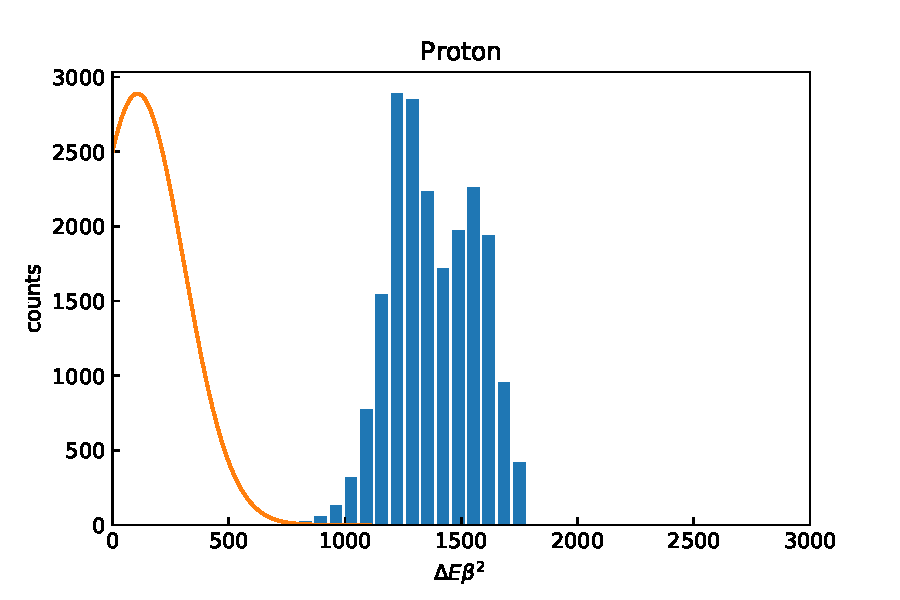
\includegraphics[width=\textwidth]{dat/debeta_Proton.pdf}
	\end{subfigure}
	\begin{subfigure}[c]{0.45\textwidth}
		\centering
		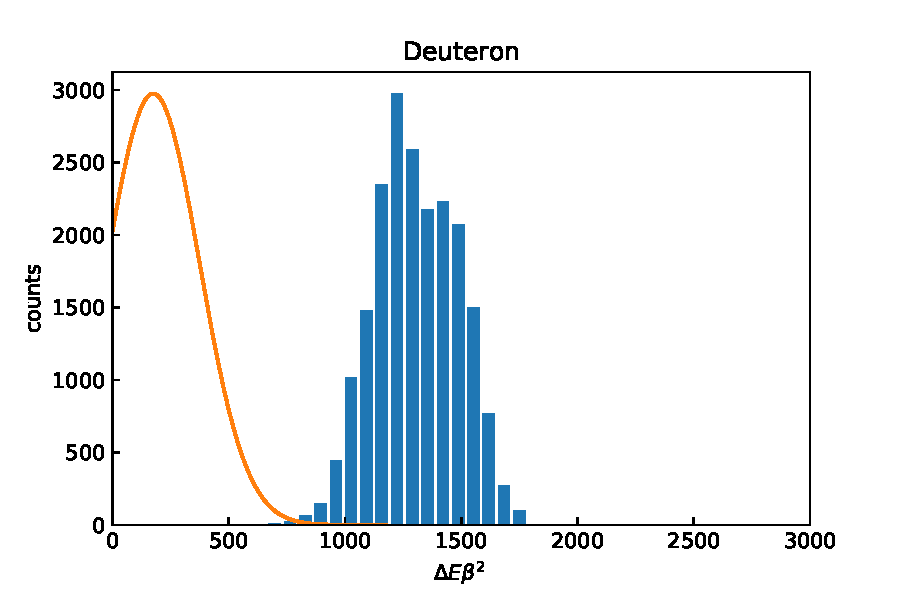
\includegraphics[width=\textwidth]{dat/debeta_Deuteron.pdf}
	\end{subfigure}
	
	\begin{subfigure}[c]{0.45\textwidth}
		\centering
		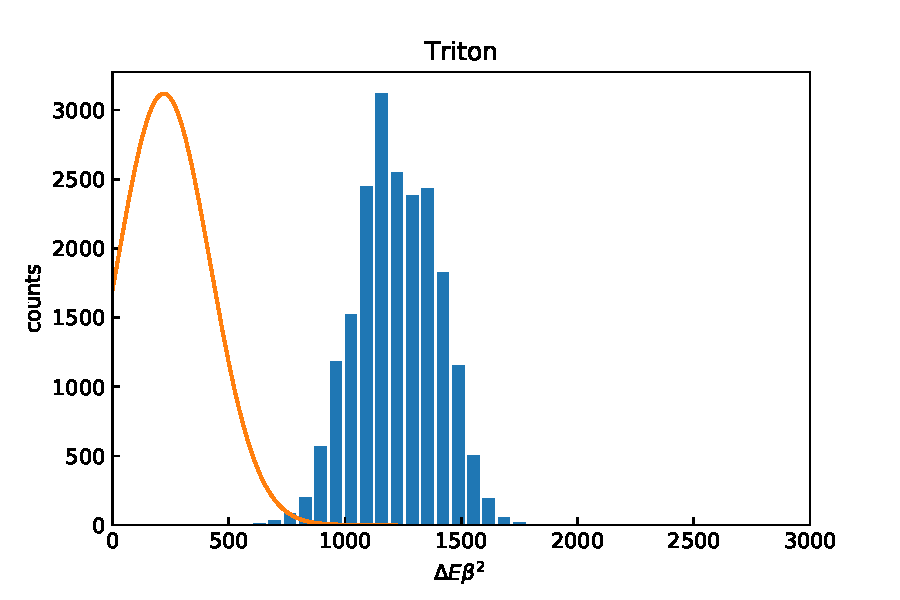
\includegraphics[width=\textwidth]{dat/debeta_Triton.pdf}
	\end{subfigure}
	\begin{subfigure}[c]{0.45\textwidth}
		\centering
		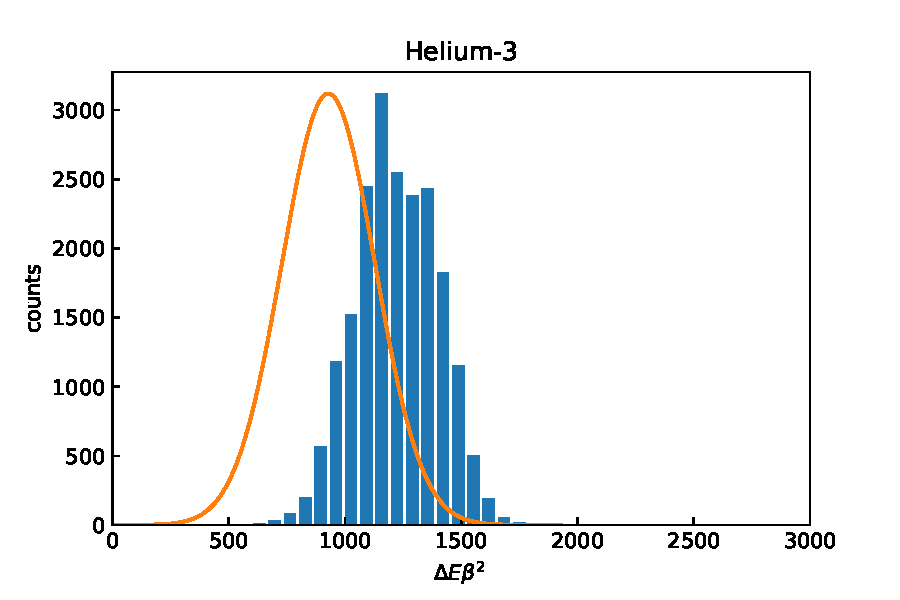
\includegraphics[width=\textwidth]{dat/debeta_Helium-3.pdf}
	\end{subfigure}
	
	\begin{subfigure}[c]{0.45\textwidth}
		\centering
		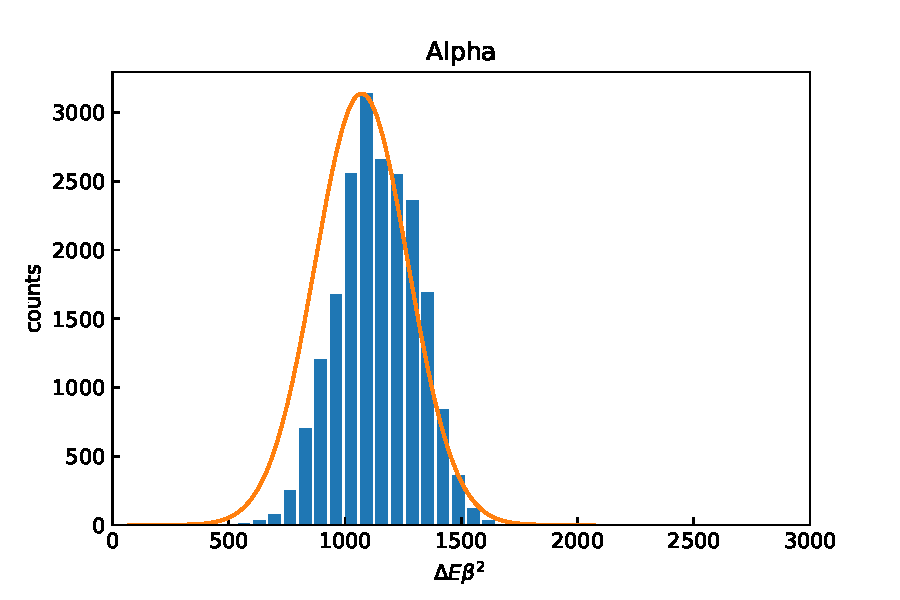
\includegraphics[width=\textwidth]{dat/debeta_Alpha.pdf}
	\end{subfigure}
	\begin{subfigure}[c]{0.45\textwidth}
		\centering
		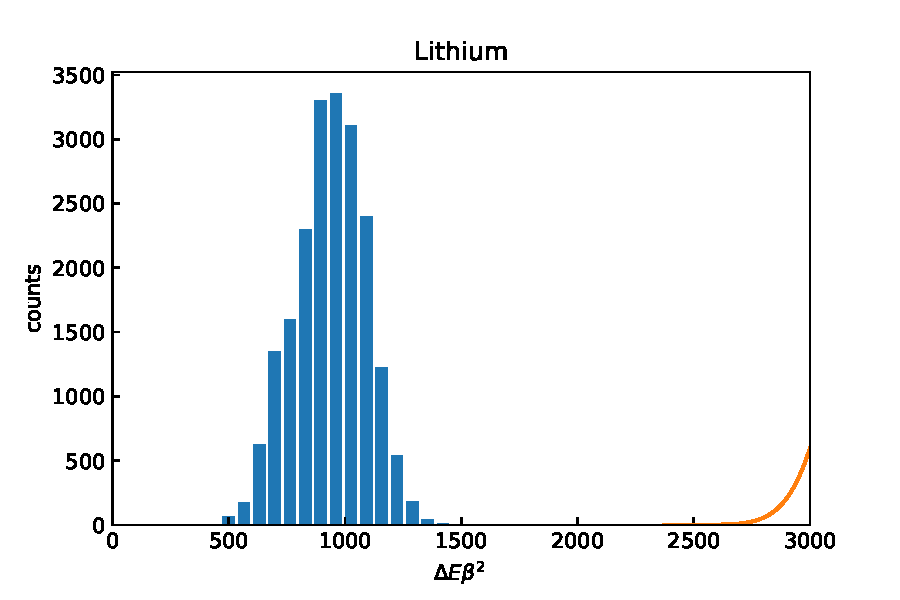
\includegraphics[width=\textwidth]{dat/debeta_Lithium.pdf}
	\end{subfigure}
	
	\caption{$\Delta E \beta^2$ Verteilungen für vermutete Teilchenarten. Eingezeichnet sind die gemessenen Werte, sowie die theoretisch zu erwartenden Verteilungen. $\alpha$-Teilchen geben die Messergebnisse am besten wieder.}
	\label{fig:debeta_full}
\end{figure}

\subsection{Fit-Parameter}
\label{sec:fitval}

\begin{table}[H]
	\centering
	\caption{Fit-Parameter für die normierte Doppelgaussfunktion \mbox{$n(E) = A_1 \cdot \exp{-\frac{(E - E_1)^2}{2 \sigma_1^2}} + A_2 \cdot \exp{-\frac{(E - E_2)^2}{2 \sigma_2^2}} + E_0$} der Dickebestimmung.}
	\label{tab:fitval1}
	\input{dat/m3_fitdaten.txt}
\end{table}